\documentclass{standalone}
\usepackage{tikz}
\usetikzlibrary{patterns, positioning}
\usetikzlibrary{shapes.misc}
\usepackage[outline]{contour}
\contourlength{1.5pt} 
\usepackage[sfdefault]{ClearSans} %% option 'sfdefault' activates Clear Sans as the default text font
\usepackage[T1]{fontenc}

\begin{document}
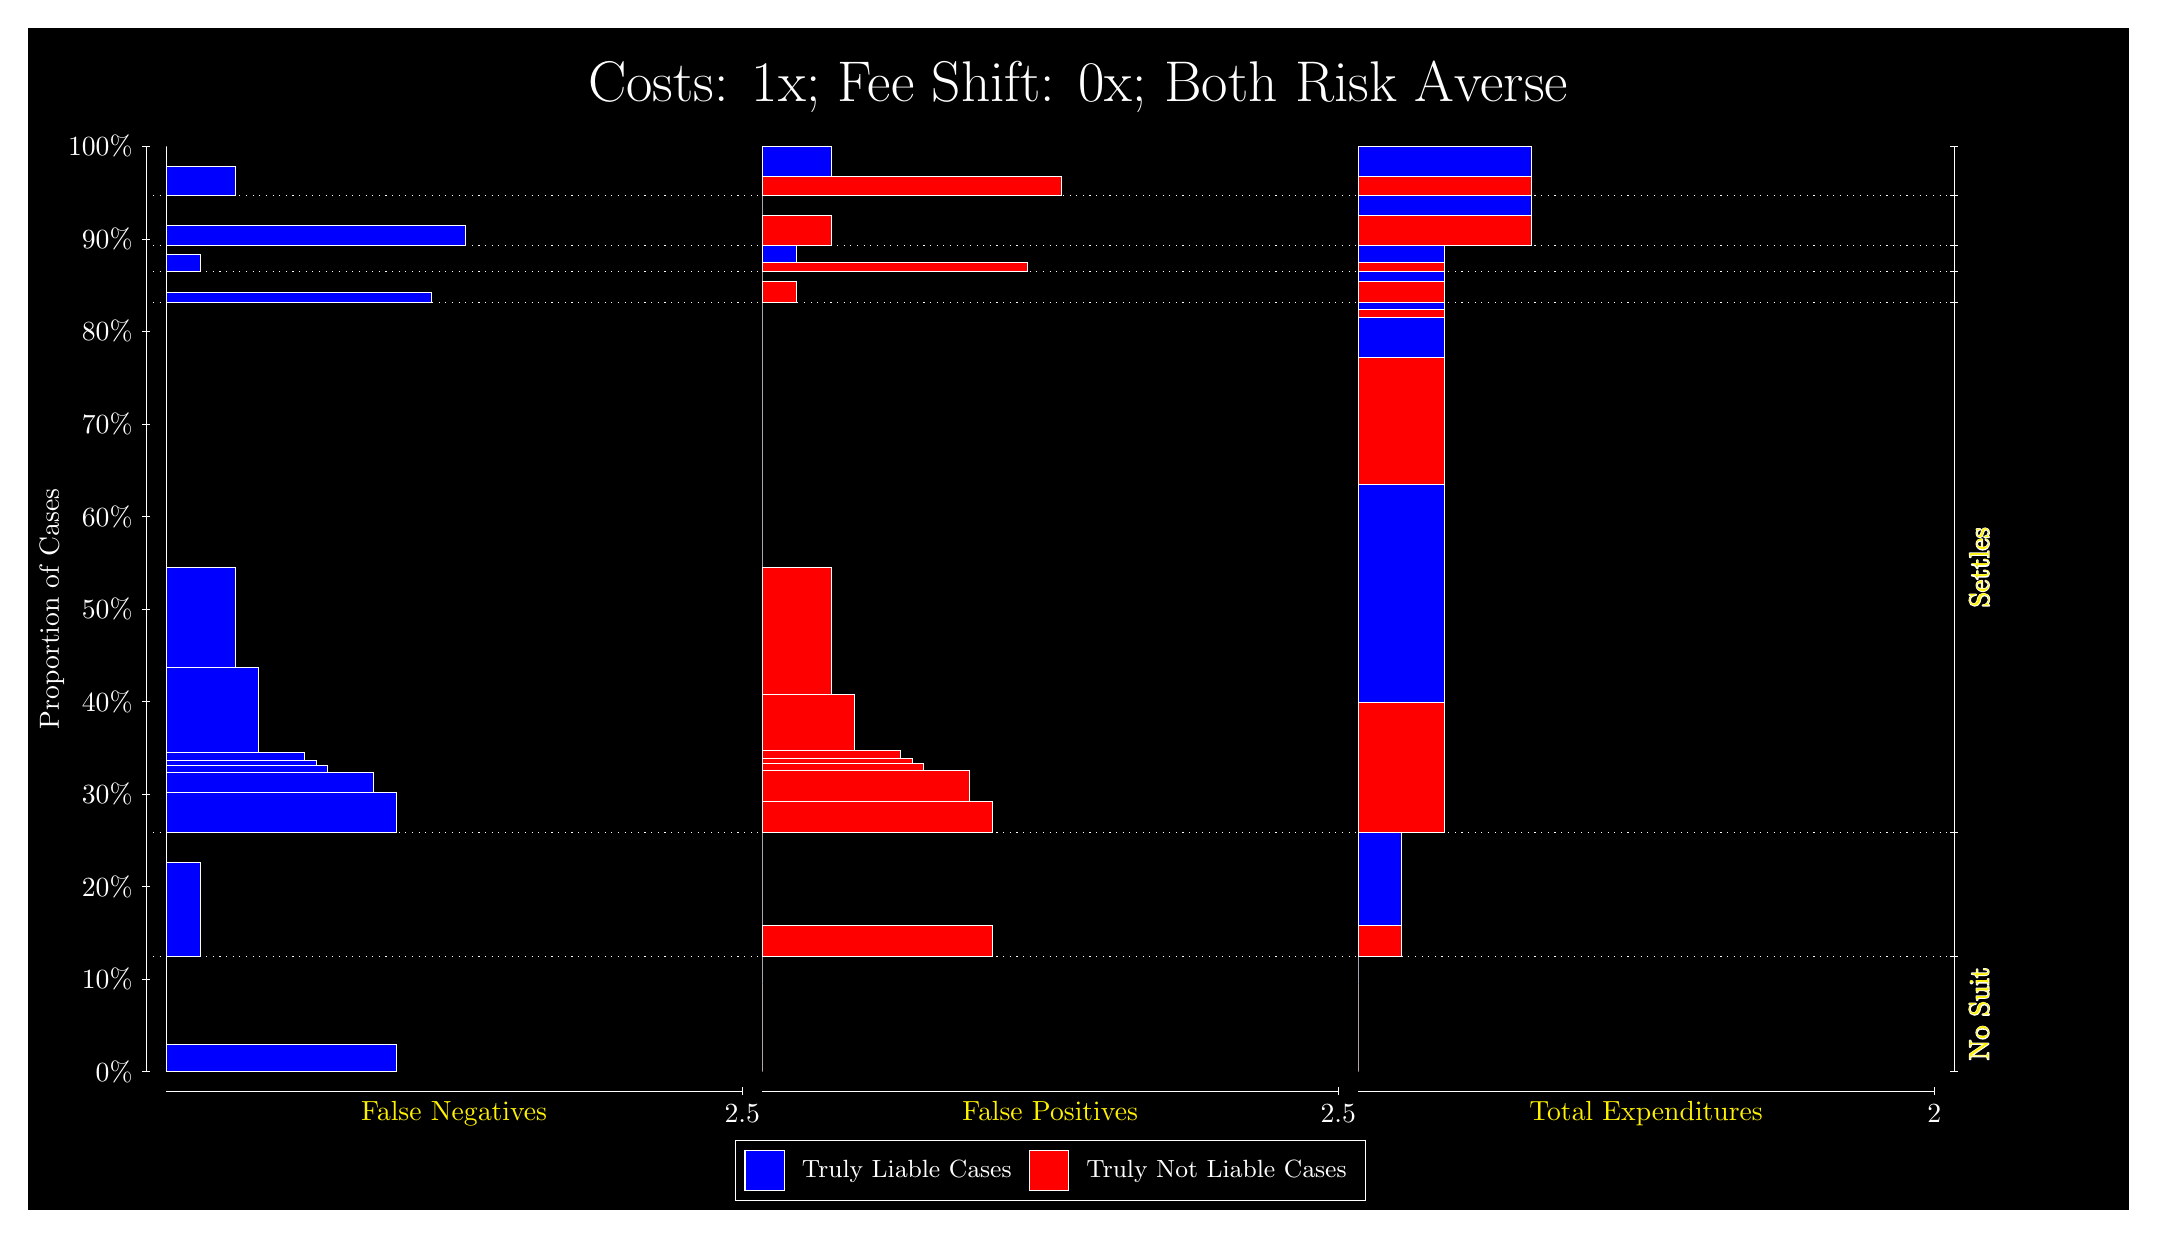
\begin{tikzpicture}
\draw[fill=black] (0,0) rectangle (26.667,15);
\draw[text=white] (0,13.5) rectangle (26.667,15) node[midway] {\huge Costs: 1x; Fee Shift: 0x; Both Risk Averse};
\draw[white, very thin] (1.5,1.75) -- (1.5,13.5);
\node[rotate=90, text=white, anchor=center] at (0.3, 7.625) {Proportion of Cases};
\draw[white, very thin] (1.45,1.75) -- (1.55,1.75);
\node[text=white, anchor=east] at (1.45, 1.75) {0\%};
\draw[white, very thin] (1.45,2.925) -- (1.55,2.925);
\node[text=white, anchor=east] at (1.45, 2.925) {10\%};
\draw[white, very thin] (1.45,4.1) -- (1.55,4.1);
\node[text=white, anchor=east] at (1.45, 4.1) {20\%};
\draw[white, very thin] (1.45,5.275) -- (1.55,5.275);
\node[text=white, anchor=east] at (1.45, 5.275) {30\%};
\draw[white, very thin] (1.45,6.45) -- (1.55,6.45);
\node[text=white, anchor=east] at (1.45, 6.45) {40\%};
\draw[white, very thin] (1.45,7.625) -- (1.55,7.625);
\node[text=white, anchor=east] at (1.45, 7.625) {50\%};
\draw[white, very thin] (1.45,8.8) -- (1.55,8.8);
\node[text=white, anchor=east] at (1.45, 8.8) {60\%};
\draw[white, very thin] (1.45,9.975) -- (1.55,9.975);
\node[text=white, anchor=east] at (1.45, 9.975) {70\%};
\draw[white, very thin] (1.45,11.15) -- (1.55,11.15);
\node[text=white, anchor=east] at (1.45, 11.15) {80\%};
\draw[white, very thin] (1.45,12.325) -- (1.55,12.325);
\node[text=white, anchor=east] at (1.45, 12.325) {90\%};
\draw[white, very thin] (1.45,13.5) -- (1.55,13.5);
\node[text=white, anchor=east] at (1.45, 13.5) {100\%};

\draw[white, very thin] (24.457,1.75) -- (24.457,13.5);
\draw[white, very thin] (24.407,1.75) -- (24.507,1.75);
\node[anchor=west] at (24.407, 1.75) {};
\draw[white, very thin] (24.407,3.2163) -- (24.507,3.2163);
\node[anchor=west] at (24.407, 3.2163) {};
\draw[white, very thin] (24.407,4.7877) -- (24.507,4.7877);
\node[anchor=west] at (24.407, 4.7877) {};
\draw[white, very thin] (24.407,11.518) -- (24.507,11.518);
\node[anchor=west] at (24.407, 11.518) {};
\draw[white, very thin] (24.407,11.913) -- (24.507,11.913);
\node[anchor=west] at (24.407, 11.913) {};
\draw[white, very thin] (24.407,12.242) -- (24.507,12.242);
\node[anchor=west] at (24.407, 12.242) {};
\draw[white, very thin] (24.407,12.872) -- (24.507,12.872);
\node[anchor=west] at (24.407, 12.872) {};
\draw[white, very thin] (24.407,13.5) -- (24.507,13.5);
\node[anchor=west] at (24.407, 13.5) {};

\draw[white, very thin, fill=blue] (1.75,1.75) rectangle (4.6775,2.0985);
\draw[white, very thin, fill=red] (1.75,2.0985) rectangle (1.75,3.2163);
\draw[white, very thin, fill=blue] (1.75,3.2163) rectangle (2.1891,4.4023);
\draw[white, very thin, fill=red] (1.75,4.4023) rectangle (1.75,4.7877);
\draw[white, very thin, fill=blue] (1.75,4.7877) rectangle (4.6775,5.2946);
\draw[white, very thin, fill=blue] (1.75,5.2946) rectangle (4.3848,5.5483);
\draw[white, very thin, fill=blue] (1.75,5.5483) rectangle (3.7993,5.6346);
\draw[white, very thin, fill=blue] (1.75,5.6346) rectangle (3.6529,5.698);
\draw[white, very thin, fill=blue] (1.75,5.698) rectangle (3.5065,5.8043);
\draw[white, very thin, fill=blue] (1.75,5.8043) rectangle (2.921,6.8847);
\draw[white, very thin, fill=blue] (1.75,6.8847) rectangle (2.6283,8.1537);
\draw[white, very thin, fill=red] (1.75,8.1537) rectangle (1.75,11.518);
\draw[white, very thin, fill=blue] (1.75,11.518) rectangle (5.1167,11.645);
\draw[white, very thin, fill=red] (1.75,11.645) rectangle (1.75,11.913);
\draw[white, very thin, fill=blue] (1.75,11.913) rectangle (2.1891,12.133);
\draw[white, very thin, fill=red] (1.75,12.133) rectangle (1.75,12.242);
\draw[white, very thin, fill=blue] (1.75,12.242) rectangle (5.5558,12.492);
\draw[white, very thin, fill=red] (1.75,12.492) rectangle (1.75,12.872);
\draw[white, very thin, fill=blue] (1.75,12.872) rectangle (2.6283,13.249);
\draw[white, very thin, fill=red] (1.75,13.249) rectangle (1.75,13.5);
\draw[white, very thin, fill=red] (9.3189,1.75) rectangle (9.3189,2.8677);
\draw[white, very thin, fill=blue] (9.3189,2.8677) rectangle (9.3189,3.2163);
\draw[white, very thin, fill=red] (9.3189,3.2163) rectangle (12.246,3.6016);
\draw[white, very thin, fill=blue] (9.3189,3.6016) rectangle (9.3189,4.7877);
\draw[white, very thin, fill=red] (9.3189,4.7877) rectangle (12.246,5.1804);
\draw[white, very thin, fill=red] (9.3189,5.1804) rectangle (11.954,5.5737);
\draw[white, very thin, fill=red] (9.3189,5.5737) rectangle (11.368,5.6599);
\draw[white, very thin, fill=red] (9.3189,5.6599) rectangle (11.222,5.7233);
\draw[white, very thin, fill=red] (9.3189,5.7233) rectangle (11.075,5.8296);
\draw[white, very thin, fill=red] (9.3189,5.8296) rectangle (10.49,6.541);
\draw[white, very thin, fill=red] (9.3189,6.541) rectangle (10.197,8.1524);
\draw[white, very thin, fill=blue] (9.3189,8.1524) rectangle (9.3189,11.518);
\draw[white, very thin, fill=red] (9.3189,11.518) rectangle (9.758,11.787);
\draw[white, very thin, fill=blue] (9.3189,11.787) rectangle (9.3189,11.913);
\draw[white, very thin, fill=red] (9.3189,11.913) rectangle (12.686,12.022);
\draw[white, very thin, fill=blue] (9.3189,12.022) rectangle (9.758,12.242);
\draw[white, very thin, fill=red] (9.3189,12.242) rectangle (10.197,12.621);
\draw[white, very thin, fill=blue] (9.3189,12.621) rectangle (9.3189,12.872);
\draw[white, very thin, fill=red] (9.3189,12.872) rectangle (13.125,13.123);
\draw[white, very thin, fill=blue] (9.3189,13.123) rectangle (10.197,13.5);
\draw[white, very thin, fill=red] (16.888,1.75) rectangle (16.888,2.8677);
\draw[white, very thin, fill=blue] (16.888,2.8677) rectangle (16.888,3.2163);
\draw[white, very thin, fill=red] (16.888,3.2163) rectangle (17.437,3.6016);
\draw[white, very thin, fill=blue] (16.888,3.6016) rectangle (17.437,4.7877);
\draw[white, very thin, fill=red] (16.888,4.7877) rectangle (17.986,6.4347);
\draw[white, very thin, fill=blue] (16.888,6.4347) rectangle (17.986,9.2076);
\draw[white, very thin, fill=red] (16.888,9.2076) rectangle (17.986,10.819);
\draw[white, very thin, fill=blue] (16.888,10.819) rectangle (17.986,11.326);
\draw[white, very thin, fill=red] (16.888,11.326) rectangle (17.986,11.432);
\draw[white, very thin, fill=blue] (16.888,11.432) rectangle (17.986,11.518);
\draw[white, very thin, fill=red] (16.888,11.518) rectangle (17.986,11.787);
\draw[white, very thin, fill=blue] (16.888,11.787) rectangle (17.986,11.913);
\draw[white, very thin, fill=red] (16.888,11.913) rectangle (17.986,12.022);
\draw[white, very thin, fill=blue] (16.888,12.022) rectangle (17.986,12.242);
\draw[white, very thin, fill=red] (16.888,12.242) rectangle (19.083,12.621);
\draw[white, very thin, fill=blue] (16.888,12.621) rectangle (19.083,12.872);
\draw[white, very thin, fill=red] (16.888,12.872) rectangle (19.083,13.123);
\draw[white, very thin, fill=blue] (16.888,13.123) rectangle (19.083,13.5);
\draw[white, dotted] (1.5,3.2163) -- (24.457,3.2163);
\draw[white, dotted] (1.5,4.7877) -- (24.457,4.7877);
\draw[white, dotted] (1.5,11.518) -- (24.457,11.518);
\draw[white, dotted] (1.5,11.913) -- (24.457,11.913);
\draw[white, dotted] (1.5,12.242) -- (24.457,12.242);
\draw[white, dotted] (1.5,12.872) -- (24.457,12.872);
\draw[white, very thin] (1.75,1.5) -- (9.0689,1.5);
\node[text=yellow, anchor=north] at (5.4094, 1.5) {False Negatives};
\draw[white, very thin] (9.0689,1.45) -- (9.0689,1.55);
\node[text=white, anchor=north] at (9.0689, 1.45) {2.5};

\draw[white, very thin] (9.3189,1.5) -- (16.638,1.5);
\node[text=yellow, anchor=north] at (12.978, 1.5) {False Positives};
\draw[white, very thin] (16.638,1.45) -- (16.638,1.55);
\node[text=white, anchor=north] at (16.638, 1.45) {2.5};

\draw[white, very thin] (16.888,1.5) -- (24.207,1.5);
\node[text=yellow, anchor=north] at (20.547, 1.5) {Total Expenditures};
\draw[white, very thin] (24.207,1.45) -- (24.207,1.55);
\node[text=white, anchor=north] at (24.207, 1.45) {2};

\node[text=yellow, centered, rotate=90] at (24.777, 2.4831) {\contour{white}{No Suit}};

\node[text=yellow, centered, rotate=90] at (24.777, 8.153) {\contour{white}{Settles}};





\draw (12.978300999999998,1.5) node[draw=none] (baseCoordinate) {};
\begin{scope}[align=center]
        \matrix[scale=0.5, draw=white, below=0.5cm of baseCoordinate, nodes={draw}, column sep=0.1cm]{
            \node[rectangle, draw, minimum width=0.5cm, minimum height=0.5cm, fill=blue] {}; &
            \node[draw=none, font=\small, text=white] (B) {Truly Liable Cases}; &
            \node[rectangle, draw, minimum width=0.5cm, minimum height=0.5cm, fill=red] {}; &
            \node[draw=none, font=\small, text=white] (B) {Truly Not Liable Cases}; \\
            };
\end{scope}

\end{tikzpicture}
\end{document}